\fullWidthTwoColumnFigureTable%
	[t] % Placement
	{0d/figures/sc_iv_uv_initial_condition.pdf} % Figure
	{fig:sc_iv_uv_initial_condition} % Figure label
	{%
		\uv{} potential $U ( \sigma )$ (red-dashed) and its first derivative $u ( \sigma ) = \partial_\sigma U ( \sigma )$ (blue, solid) of test case IV from \cref{eq:testing_scenario_4}. 
		\fromFig{30}{zerod1}%
	} % Figure caption
	{%
		\renewcommand{\arraystretch}{1.15}
		\small
		\begin{tabular}{l c c c}
			\toprule
			$N$		&	$\Gamma^{(2)}$	&	$\Gamma^{(4)}$	&	$\Gamma^{(6)}$	\\
			\midrule
			$1$	&	$0.204698$	&	$0.064682$	&	$0.112849$\\
			$3$	&	$0.421674$	&	$0.153559$	&	$0.249252$\\
			\bottomrule
		\end{tabular}
	} % Table content
	{tab:sc_4_n_point_functions_exact}% Table label
	{%
		Exact results for $\Gamma^{(2n)}$ of the $O(N)$ model with the \uv{} initial potential \eqref{eq:testing_scenario_4} for selected $N$.
		They are obtained by a high-precision one-dimensional numerical integration of the expectation values $\langle ( \vec{\phi}^{\, 2} )^n \rangle$ from \cref{eq:ON_expectation_value} using \textit{NIntegrate} in \WAMXIIwR{}.
		Here, we present the first six digits only.
		\textit{In parts from Tab. IV of \ccite{zerod1} and Tab. I of \ccite{zerod2}.}%
	} % Table caption
\subsubsection{Test case IV: The \texorpdfstring{$\sigma\mkern-2mu=\mkern-2mu0$}{sigma=0} boundary}
\label{subsubsec:sc4}
The last test case is again a non-analytic and discontinuous potential,
\begin{align}
	U ( \vec{\varphi} \vts ) =
	\begin{cases}
		- ( \vec{\varphi}^{\vts 2} )^{\tfrac{1}{3}} \, ,			&	\text{if} \quad |\vec{\varphi}| \leq \sqrt{8} \, ,\\
		\tfrac{1}{2} \, \vec{\varphi}^{\vts 2} - 6 \, ,							&	\text{if} \quad |\vec{\varphi}| > \sqrt{8} \, .
	\end{cases}	\label{eq:testing_scenario_4}
\end{align}
The numerically challenging features are the cusp at $\varphi = 0$ as well as a non-trivial minimum at the kink at $\varphi = \sqrt{8}$.
As displayed in \cref{fig:sc_iv_uv_initial_condition} (evaluated on the constant field configuration), the cusp\footnote{
	Potentials with cusps in field space are not just academic thought experiments.
	They are encountered in, \eg{}, theories in $2+1$ space-time dimensions, such as the Gross-Neveu model~\cite{Braun:2010tt}.
} at $\sigma = 0$ in $U(\sigma)$ translates to a pole in $\partial_\sigma U(\sigma)\equiv u(\sigma)$.
This scenario was engineered as an extreme test case for the boundary condition at $\sigma = 0$ discussed at length in \cref{paragraph:BC0}.

We have again performed the full set of numerical tests of \cref{subsubsec:sc1} and found results supporting the general statements made in \cref{subsubsec:sc1}.
For brevity, we will not repeat the complete discussion of that subsubsection but instead focus again on selected results.\bigskip

\subcaptionFigureOneTwo%
	[!t]% placement
	{0d/figures/sc_iv_on_3_n_800_xmax_10_lambda_1e8_tir_60_rg_flow.pdf}% figure (a)
	{%
		\caption{
			The \frg{} flow of the effective potential $U ( t, \sigma )$ (upper panel) and its derivative $u ( t , \sigma ) = \partial_\sigma U ( t , \sigma )$ (lower panel) evaluated at $t = 0, \, 2, \, 4, \, \ldots, \, 60$ (integer values for $t$ were chosen for convenience and readability). 
			The (overlapping) {blue} and {violet} curves correspond to the \uv{} and the {red} curves to the \ir{}.
			We used the exponential regulator~\eqref{eq:exponential_regulator} with \uv{} scale $\Lambda = 10^{8}$ and $n = 800$ volume cells.
			The plot does not show the region ${x \in[5,10]}$, because the tiny differences between $u ( t, \sigma )$ and $u ( t_\mathrm{UV}, \sigma )$ are not visible in this region and vanish for large $x = \sigma$ anyhow.
		}%
		\label{fig:sc_iv_on_3_n_800_xmax_10_lambda_1e8_tir_60_rg_flow}%
	}% caption/label (a)
	{%
		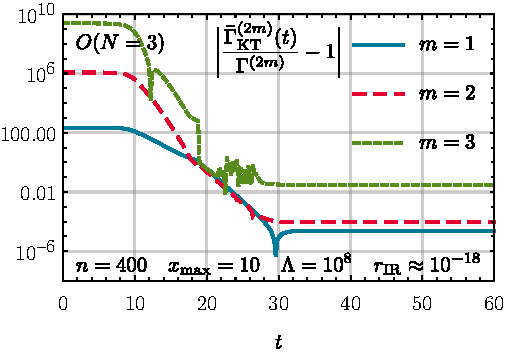
\includegraphics[width=\subcaptionFigureWidth]{0d/figures/sc_iv_on_3_n_400_xmax_10_lambda_1e8_tir_60_flow_errors.pdf}
		\caption{
			The relative error for $\Gamma^{(2m)}(t)$, for $m = 1, 2$, calculated with the \ktScheme{} as a function of the \rgtime{} $t$ for the $O(3)$ model.
			We used the exponential regulator~\eqref{eq:exponential_regulator} with \uv{} scale $\Lambda = 10^{8}$ and $n = 400$ volume cells.
		}%
		\label{fig:sc_iv_on_3_n_400_xmax_10_lambda_1e8_tir_60_flow_errors}%
	}% figure/caption/label (b)
	{%
		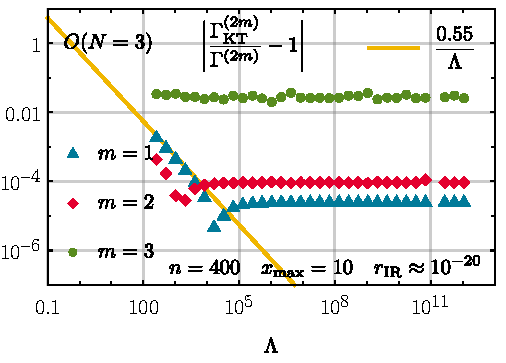
\includegraphics[width=\subcaptionFigureWidth]{0d/figures/sc_iv_on_3_n_400_xmax_10_rir_10e-20_cutoff_test.pdf}
		\caption{
			The relative error for $\Gamma^{(2m)}(t_\mathrm{IR})$ for $m = 1, 2, 3$ from the \ktScheme{} as a function of the \uv{} scale scale $\Lambda$.
			We use the exponential regulator~\eqref{eq:exponential_regulator} and keep the \ir{} cutoff scale constant at $r(t_\mathrm{IR}) = 10^{-15}$ for all runs.
			The number of volume cells is $n = 400$.
			The straight yellow line $\propto \Lambda^{-1}$ is for optical guidance.
		}%
		\label{fig:sc_iv_on_3_n_400_xmax_10_rir_10e-20_cutoff_test}%
	}% figure/caption/label (c)
	{%
		\Frg{} flow on the left \subref{fig:sc_iv_on_3_n_800_xmax_10_lambda_1e8_tir_60_rg_flow}, relative errors over \rgtime{} on the top right \subref{fig:sc_iv_on_3_n_400_xmax_10_lambda_1e8_tir_60_flow_errors}, and relative errors in the \ir{} as function of the \uv{} cutoff $\Lambda$ on the bottom right \subref{fig:sc_iv_on_3_n_400_xmax_10_rir_10e-20_cutoff_test} for the zero-dimensional $O ( 3 )$ model with initial condition \cref{eq:testing_scenario_4}.
		The computational grid size is $\sigma_\mathrm{max} = x_\mathrm{max} = 10$ and $\Gamma^{(2m)}(t)$ are calculated from $u ( t, \sigma )$ via the approximations \eqref{eq:derivative_1_central_error_2}, \eqref{eq:derivative_3_central_error_2}, and \eqref{eq:derivative_5_central_error_2} for the numerical derivatives.
		\fromFigs{31, 32, and 33}{zerod1}%
	}% caption
	{fig:sc_iv_flows}% label
\Cref{fig:sc_iv_on_3_n_800_xmax_10_lambda_1e8_tir_60_rg_flow} depicts the \frg{} flow for the $O(3)$ model computed with the \ktScheme{} for the \uv{} initial condition \eqref{eq:testing_scenario_4}.
\Cref{fig:sc_iv_on_3_n_400_xmax_10_lambda_1e8_tir_60_flow_errors} displays the corresponding flow of the first three non-vanishing \nptFunctions{}.
With our implementation of the \ktScheme{} using \textit{NDSolve} of \WAMXIIwR{} with a \textit{PrecisionGoal} and \textit{AccuracyGoal} of $10$ we are able to compute precise solutions, where the achievable precision for $\Gamma^{(4)}$ and $\Gamma^{(6)}$ is, as discussed in the previous subsubsections, limited by the finite-difference rounding errors.
The discretization-error scaling shows the same peculiarities as the test case I of \cref{subsubsec:sc1} due to the discontinuities in the initial conditions.
The corresponding  reference values for the $O(3)$ model are listed in \cref{tab:sc_4_n_point_functions_exact}.
The dynamics during the \frg{} flow is dominated by the pole at $\sigma = 0$ and the discontinuity at $\sigma = \sqrt{8}$ in $u(\sigma)$.
The diffusion smears out the discontinuity and advection transports it towards $\sigma = 0$ ``filling up the well'' at $\sigma = 0$.
Considering the corresponding values for $u(\sigma)$ for $\sigma < 0$ using the antisymmetry of $u(\sigma)$, the boundary at $\sigma = 0$ can be seen as a point where waves of opposite amplitude annihilate \dash{} a situation very reminiscent of our discussion of the \bbeq{} in \cref{paragraph:BBE}.

Only the carefully engineered boundary condition at $\sigma = 0$ together with corresponding ghost cells allows for practical computations with the present initial condition.
The pole at $\sigma = 0$ presents no problem in practical computations because the boundary condition at $\sigma = 0$ makes use of the antisymmetry of $u ( t, \sigma )$. 
The first cell containing the pole is centered at $\sigma = 0$ and due to the antisymmetry, the corresponding cell average $\bar{u}_0(t)$ vanishes by construction.
Enforcing $\bar{u}_0(t)=0$ and for the two ghost cells $\bar{u}_{-2}(t)=-\bar{u}_{2}(t)$ and $\bar{u}_{-1}(t)=-\bar{u}_{1}(t)$ at each time step allows for a stable and accurate \frg{} time evolution even for such extreme initial conditions like the one of \cref{eq:testing_scenario_4}.

Treating this initial condition using a formulation in the invariant $\varrho = \tfrac{1}{2} \, \sigma^2$ with some naive boundary conditions without strict mathematical justification is hazardous, because $u ( t, \varrho ) = \partial_\varrho U ( t, \varrho )$ diverges as $\varrho^{-2/3}$ as $\varrho \rightarrow 0$.
As mentioned in \cref{paragraph:BC0}, it is unclear to us how to deal with the $\varrho = 0$ boundary especially in a case like the one discussed in this subsubsection.\bigskip

We conclude this subsection with a short discussion of \rgcy{}.
The plateaus in \cref{fig:sc_iv_on_3_n_400_xmax_10_lambda_1e8_tir_60_flow_errors} in the \uv{} (at small $t$) and the \ir{} (at large $t$) are again a strong indication for appropriately chosen \uv{} and \ir{} scales.
From \cref{fig:sc_iv_on_3_n_400_xmax_10_rir_10e-20_cutoff_test}, showing the $\Lambda$-dependence of $\Gamma^{(2)}$, $\Gamma^{(4)}$, and $\Gamma^{(6)}$, one observes that, even in the presence of the pole at $\sigma = 0$ in ${u ( t = 0, \sigma )}$, an initial \uv{} scale of $\Lambda=10^8$ is sufficient to realize \rgcy{}. 
Arguably even $\Lambda=10^6$ \dash{} the scale used in \cref{subsubsec:sc1} \dash{} would suffice, suggesting that in the current case the scale is primarily set by the discontinuity and linear asymptotics at and beyond $\sigma = \sqrt{8}$, which both are also present (with very similar values) in the initial condition \eqref{eq:testing_scenario_non-analytic_quadaratic_asymptote} of \cref{subsubsec:sc1}.

However, decreasing $\Delta x$ would lead to larger numerical gradients for the initial condition at $\sigma = 0$ due to the discretization of the pole in $u(\sigma)$, which in turn implies that $\Lambda$ has to be simultaneously increased in order to keep the propagators \eqref{eq:advection_flux_pion_propagator} and \eqref{eq:diffusion_flux_sigma_propagator} dominated by $\Lambda$ in the \uv{}.

Also, if the cusp at $\sigma = 0$ in the \uv{} initial potential $U ( t = 0, \sigma )$ in \cref{fig:sc_iv_uv_initial_condition} pointed downwards and $u ( 0, x )$ had negative gradients on both sides of the corresponding pole, it would formally be extremely hard to guarantee the inequalities \eqref{eq:LambdaMin} and to have a non-singular flow equation in the \uv{}, because the giant negative gradients would not be restricted to the cell at $\sigma = 0$.
In a discretized version with non-zero $\Delta x$ a calculation is still possible, as long as $\Lambda$ is chosen extremely large, much larger than the huge, but finite negative gradient of $u(\sigma)$.
Hence, \rgcy{} is not only a physical requirement, but also sets strict limits on the choice of numerical parameters, respectively.
We observe similar effects in \cref{paragraph:chemical_potential_shock_wave}, where the chemical potential enters as a shock wave in field space with (at $T=0$) infinite negative slope in $u(t,\sigma)$ at positive $\sigma$.